\chapter{Design Approach} \label{chap:designaproach}
%%%%%%Intoduction/description
Based on the requirements mentioned in Section \ref{sec:requirements} the approach shown in \autoref{fig:controllerDiagram} is designed to autonomously survey an area specified by four pairs of coordinates given in the NED frame, \{$x_\mathrm{n}$; $y_\mathrm{n}$\}.
\begin{figure}[H]
    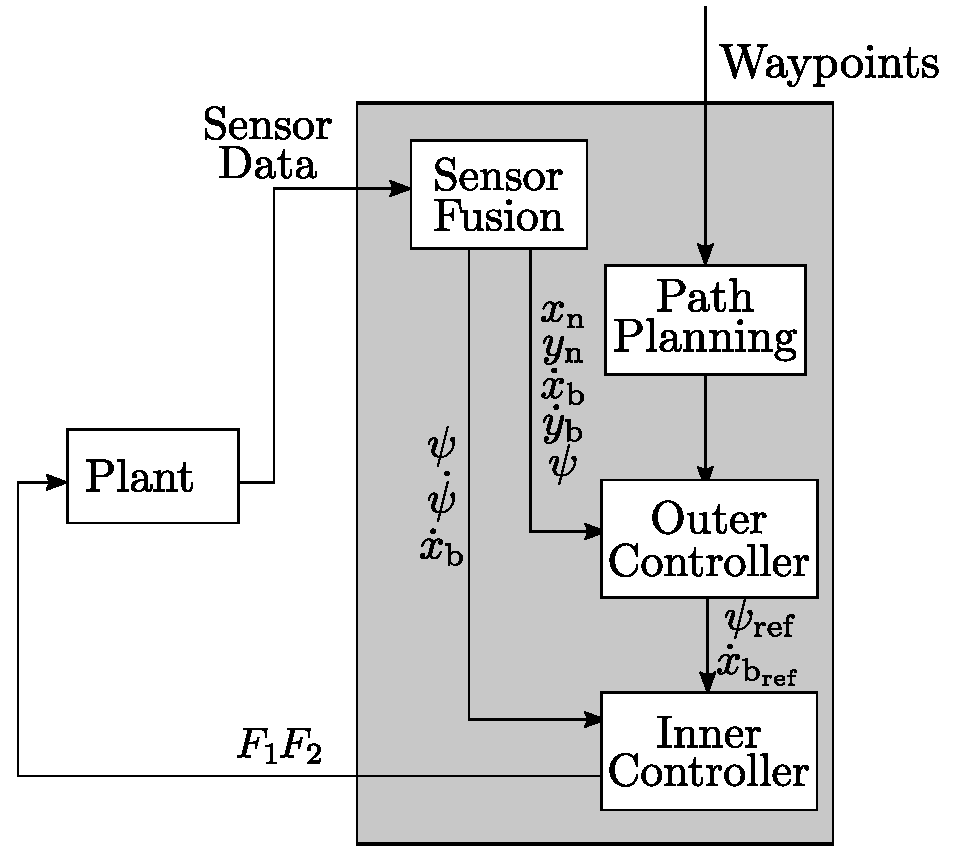
\includegraphics[width=0.42\textwidth]{figures/controllerDiagram2}
    \caption{Diagram of the control approach.}
    \label{fig:controllerDiagram}
\end{figure}

This is achieved by computing a path within the specified area, based on a predefined width, to perform bathymetric measurements. The path is used as input into the controllers, making the vessel follow it. 

%%%%% Path generation
The control design consists of two controllers, an inner controller and an outer controller. These work in the two coordinate frames, described in \autoref{sec:frames}.

As shown in \autoref{fig:controllerDiagram} the outer controller is in charge of following the path by changing the reference of the inner controller. Using the position of the vessel in the NED frame, $x_\mathrm{n}$ and $y_\mathrm{n}$, as well as its velocity in the body frame, $x_\mathrm{b}$ and $y_\mathrm{b}$, it is able to compute the $\psi_\mathrm{ref}$ and $\dot{x}_\mathrm{b,ref}$ needed to follow the path. 

The inner controller uses these references to control $\dot{x}_\mathrm{b}$ and $\dot{\psi}$ by asking for the appropriate $F_1$ and $F_2$ commands. Two design approaches are tested for the inner controller, an $H_{\infty}$ controller and a linear quadratic regulator (LQR).

The $H_{\infty}$ controller is designed to be robust towards wind, current and wave disturbances and towards model errors. The LQR, on the other side, is designed to minimize a cost function that depends on the states and on the usage of inputs. The two approaches for the inner controller are then tested in simulation, to compare the robustness and performance of both of them.

%%%%%Sensor Fusion%%%%%%
Additionally, to improve the precision of the measurements, the sensor data is fused together before it is used as input for the controllers. Two Kalman filters, based on the model of the vessel, are used to filter the measurements. One estimates the attitude variables, $\psi$ and $\dot{\psi}$, and the other the translational variables, $x_\mathrm{n}$, $y_\mathrm{n}$, $\dot{x}_\mathrm{b}$ and $\dot{y}_\mathrm{b}$.

In \autoref{chap:innercontrol} the inner controller design is included while the outer control is described in \autoref{chap:outerController}. The sensor fusion is then presented in \autoref{chap:sensorFusion}.

